\usetikzlibrary{calc}




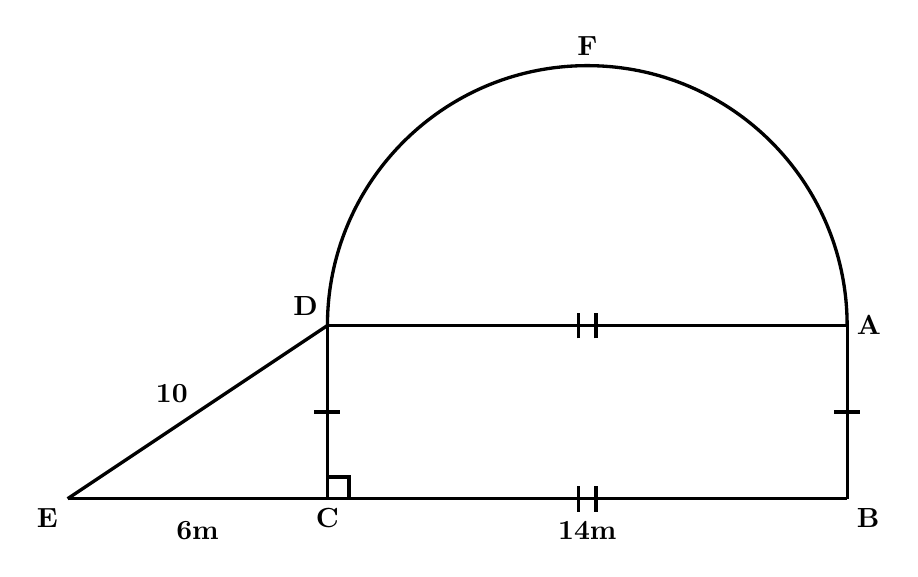
\begin{tikzpicture}[scale=0.55]
    % Define coordinates
    \coordinate (E) at (0,0);
    \coordinate (C) at (6,0);
    \coordinate (B) at (18,0);
    \coordinate (D) at (6,4);
    \coordinate (A) at (18,4);
    
    % Draw the base line E-C-B
    \draw[very thick] (E) -- (B);
    
    % Draw left slanted line E-D
    \draw[very thick] (E) -- (D);
    
    % Draw vertical line C-D
    \draw[very thick] (C) -- (D);
    
    % Draw horizontal line D-A
    \draw[very thick] (D) -- (A);
    
    % Draw vertical line A-B
    \draw[very thick] (A) -- (B);
    
    % Draw semicircle from D to A with F at top (radius = 6)
    \draw[very thick] (D) arc (180:0:6);
    
    % Right angle at C
    \draw[very thick] (C) rectangle ++(0.5,0.5);
    
    % Single tick mark on CD
    \draw[very thick] (5.7,2) -- (6.3,2);
    
    % Single tick mark on AB
    \draw[very thick] (17.7,2) -- (18.3,2);
    
    % Double tick marks on DA
    \draw[very thick] (11.8,3.7) -- (11.8,4.3);
    \draw[very thick] (12.2,3.7) -- (12.2,4.3);
    
    % Double tick marks on CB
    \draw[very thick] (11.8,-0.3) -- (11.8,0.3);
    \draw[very thick] (12.2,-0.3) -- (12.2,0.3);
    
    % Labels with bold font
    \node[below left, font=\bfseries] at (E) {E};
    \node[below, font=\bfseries] at (C) {C};
    \node[below right, font=\bfseries] at (B) {B};
    \node[above left, font=\bfseries] at (D) {D};
    \node[right, font=\bfseries] at (A) {A};
    \node[above, font=\bfseries] at (12,10) {F};
    
    % Measurements
    \node[above left, font=\bfseries] at (3,2) {10};
    \node[below, font=\bfseries] at (3,-0.3) {6m};
    \node[below, font=\bfseries] at (12,-0.3) {14m};
\end{tikzpicture}